\section{System Model}
\label{system_model}

Task service in the vehicle--RSU--UAV--cloud network depends on
communication, on motion and on how much energy is left. We model these
parts separately so that their interaction within one time slot can be
followed step by step. Fig.~\ref{fig:network_slot} gives the topology and the
execution order, and Fig.~\ref{fig:service_graph} traces one task through its
service stages. The remaining subsections define mobility, arrivals,
offloading, radio service, computation, queues, flight and battery
replenishment; Section~\ref{problem_formulation} then uses them to state the
long-term control problem.

\subsection{Network Architecture and Time-Slot Model}
\label{subsec:network_model}
The network operates over a bounded rectangular service region
$\mathcal A\subset\mathbb R^2$. Its node sets are
$\mathcal V=\{1,\ldots,V\}$ for vehicles,
$\mathcal R=\{1,\ldots,R\}$ for fixed RSUs, and
$\mathcal U=\{1,\ldots,U\}$ for rotary-wing UAV edge servers;
$c$ denotes a remote cloud. Vehicle and RSU positions are
$\boldsymbol p_v(t)=[x_v(t),y_v(t),0]^{\mathsf T}$ and
$\boldsymbol p_r=[x_r,y_r,0]^{\mathsf T}$, while UAV position and
velocity are $\boldsymbol p_k(t)\in\mathbb R^3$ and
$\boldsymbol u_k(t)\in\mathbb R^3$.

Time is divided into slots $t\in\{0,1,\ldots\}$ of duration $\Delta>0$.
At the start of slot $t$, the observed state includes the queues, the
eligible task records, node positions, UAV velocities, the physical battery
charge, the virtual energy deficits, and summaries of the current channels.
Each slot proceeds in five steps:
\begin{enumerate}
\item the start-of-slot state is observed and control proposals are generated;
\item the proposals are repaired, and radio, CPU, and flight service are
executed using only the work that was eligible when the slot began;
\item stage transfers that finished are committed at the slot boundary;
\item external tasks and the realized harvested energy are added; and
\item completions, deadline crossings, the cost, and the transition are
recorded.
\end{enumerate}
A transfer that completes in slot $t$ can therefore be served downstream in
slot $t+1$ at the earliest.

\begin{figure*}[!t]
\centering
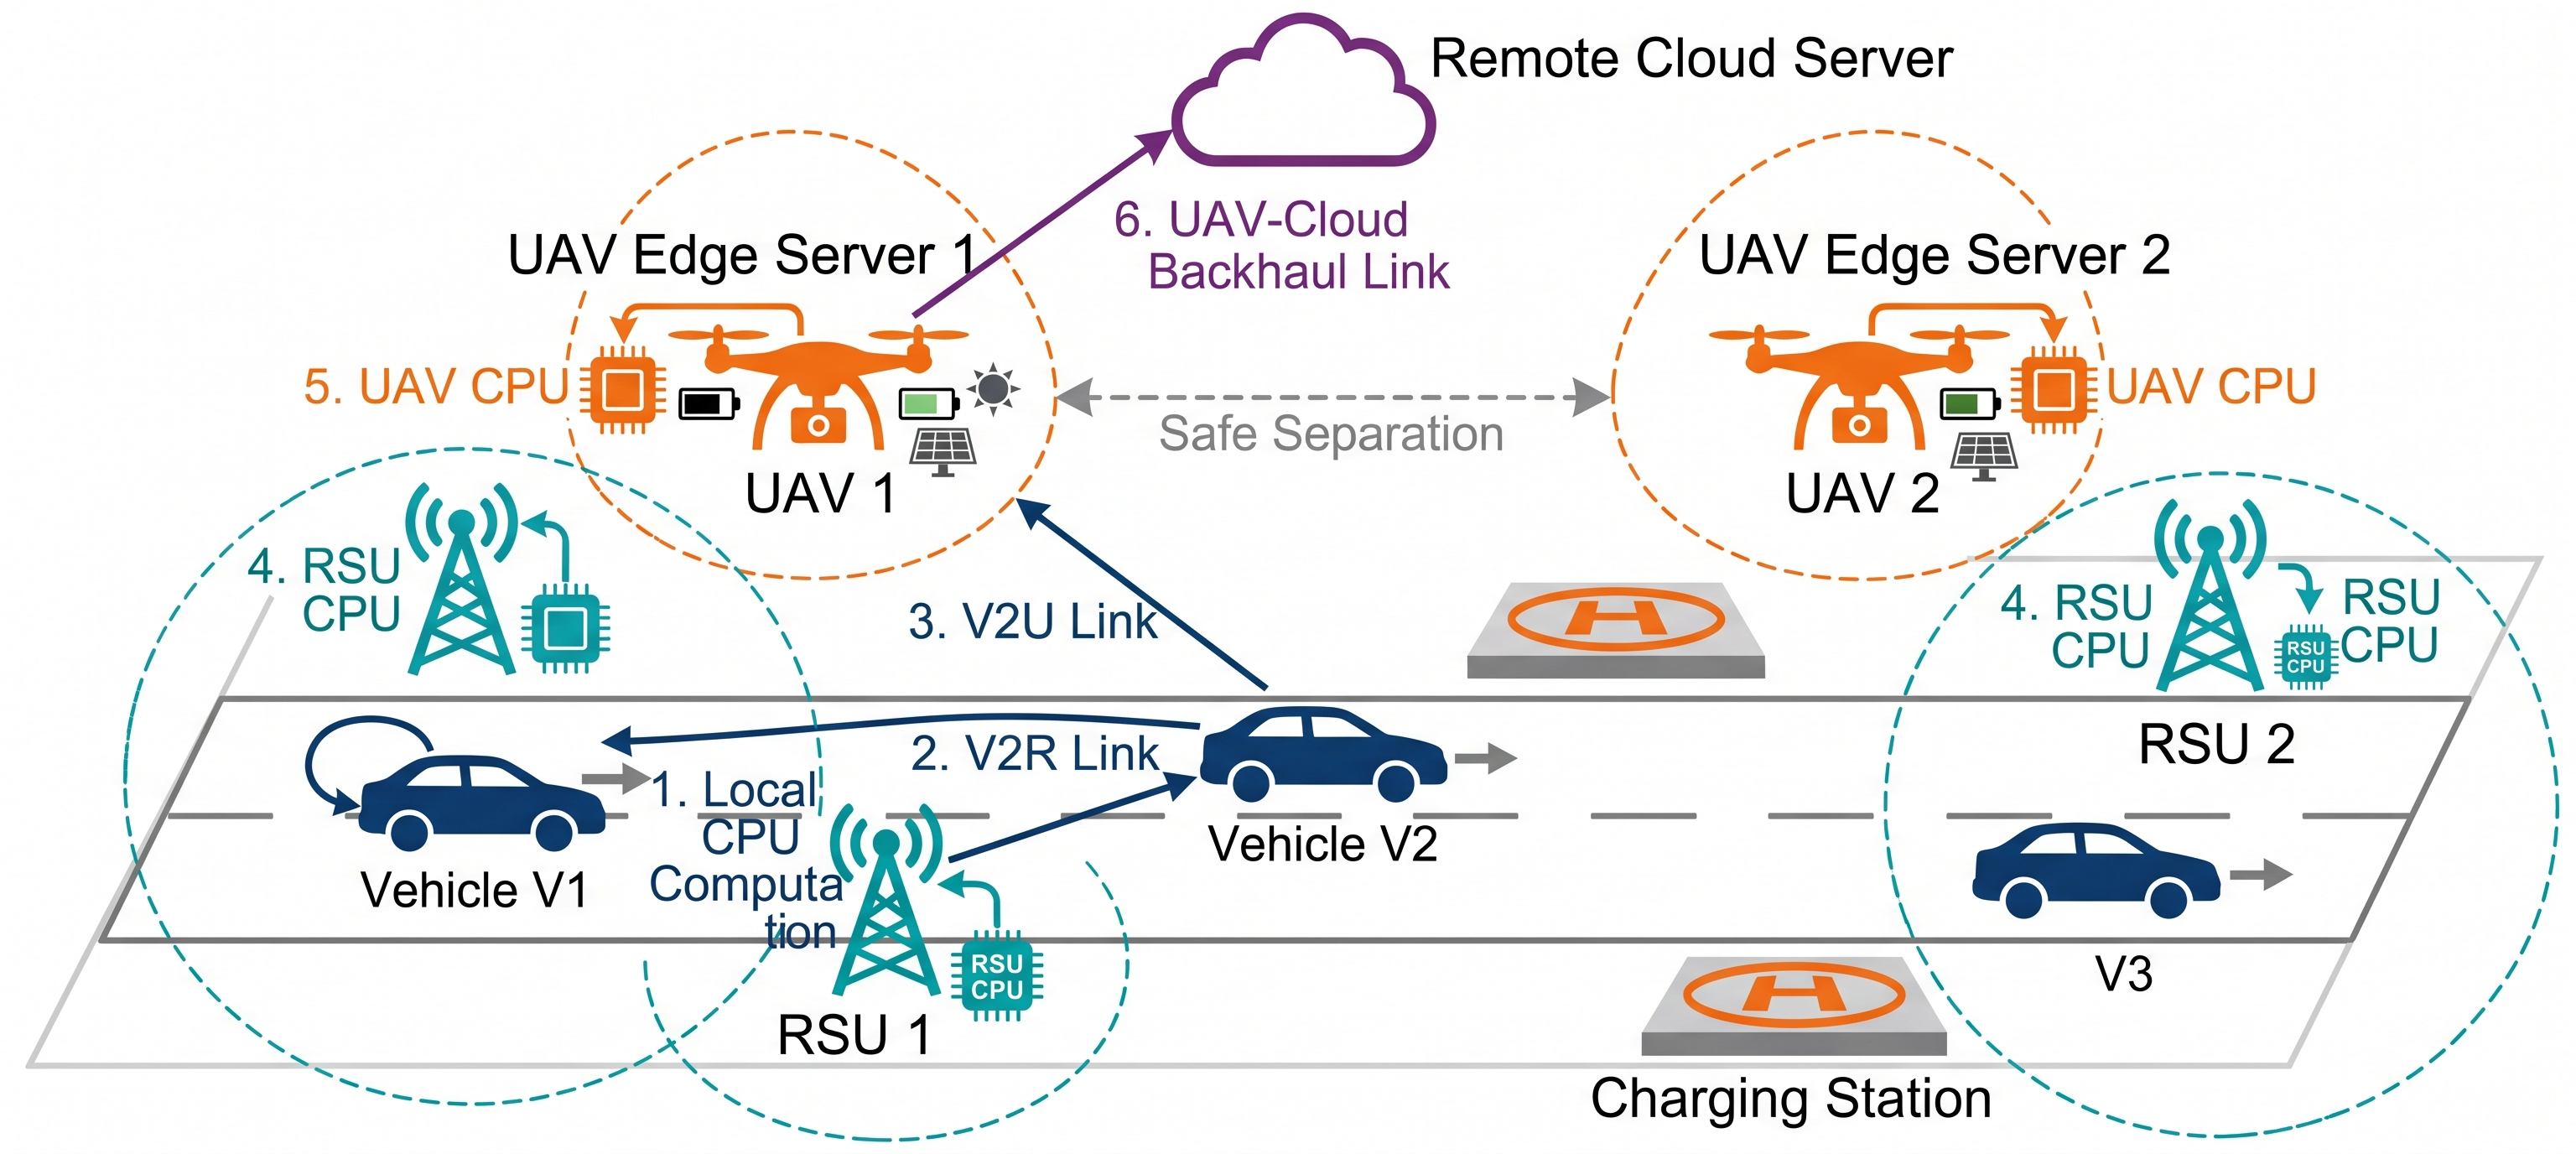
\includegraphics[width=0.94\textwidth]{Network architecture diagram.png}
\par\vspace{2pt}
{\footnotesize (a) Vehicle--RSU--UAV--cloud architecture.\par}
\vspace{5pt}
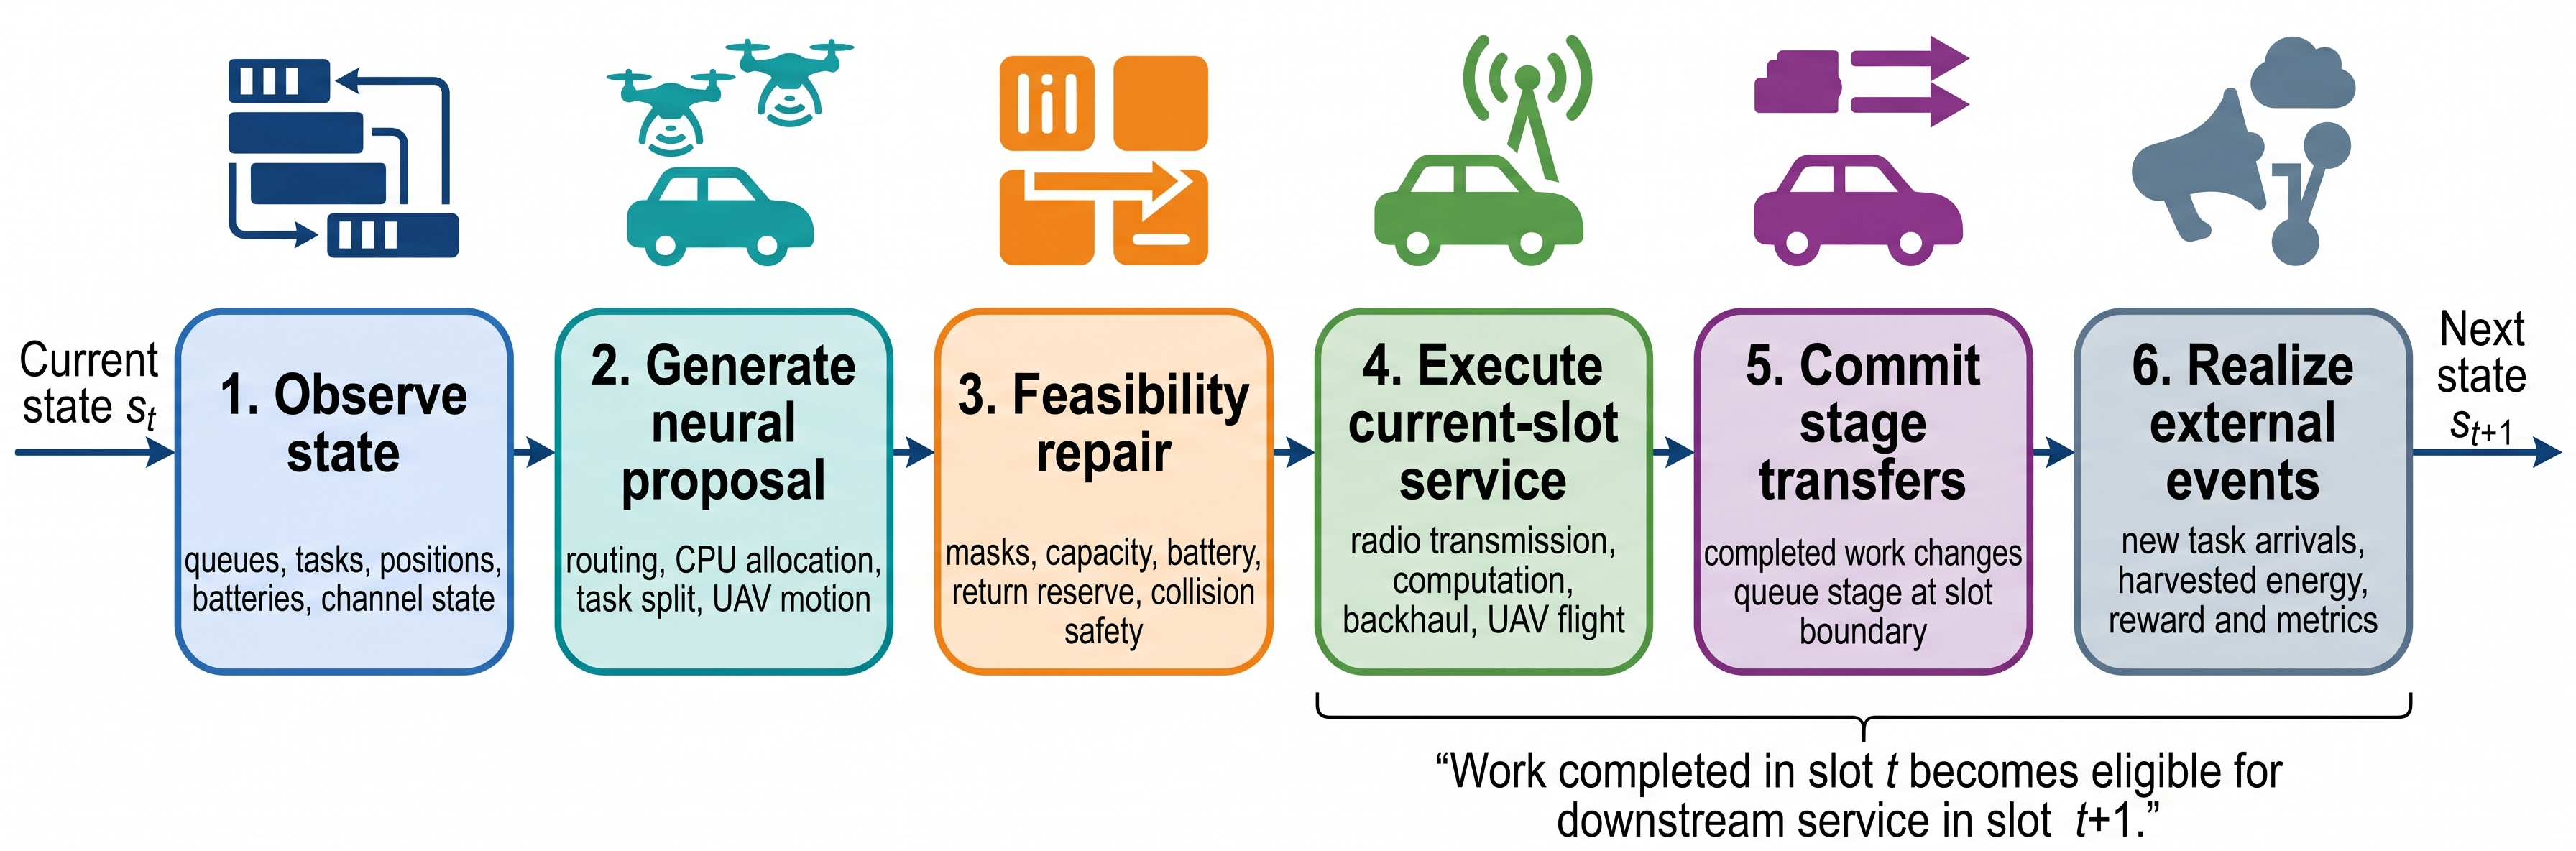
\includegraphics[width=0.96\textwidth]{Causal time-slot execution workflow.png}
\par\vspace{2pt}
{\footnotesize (b) Causal execution order within slot $t$.\par}
\caption{System architecture and causal slot execution. RSUs supply fixed
edge capacity and UAVs supply mobile edge service; work sent to a UAV may
keep a finite cloud branch. Harvested energy and external arrivals are
committed only after the service and expenditure of the current slot.}
\label{fig:network_slot}
\end{figure*}

\begin{figure*}[t]
\centering
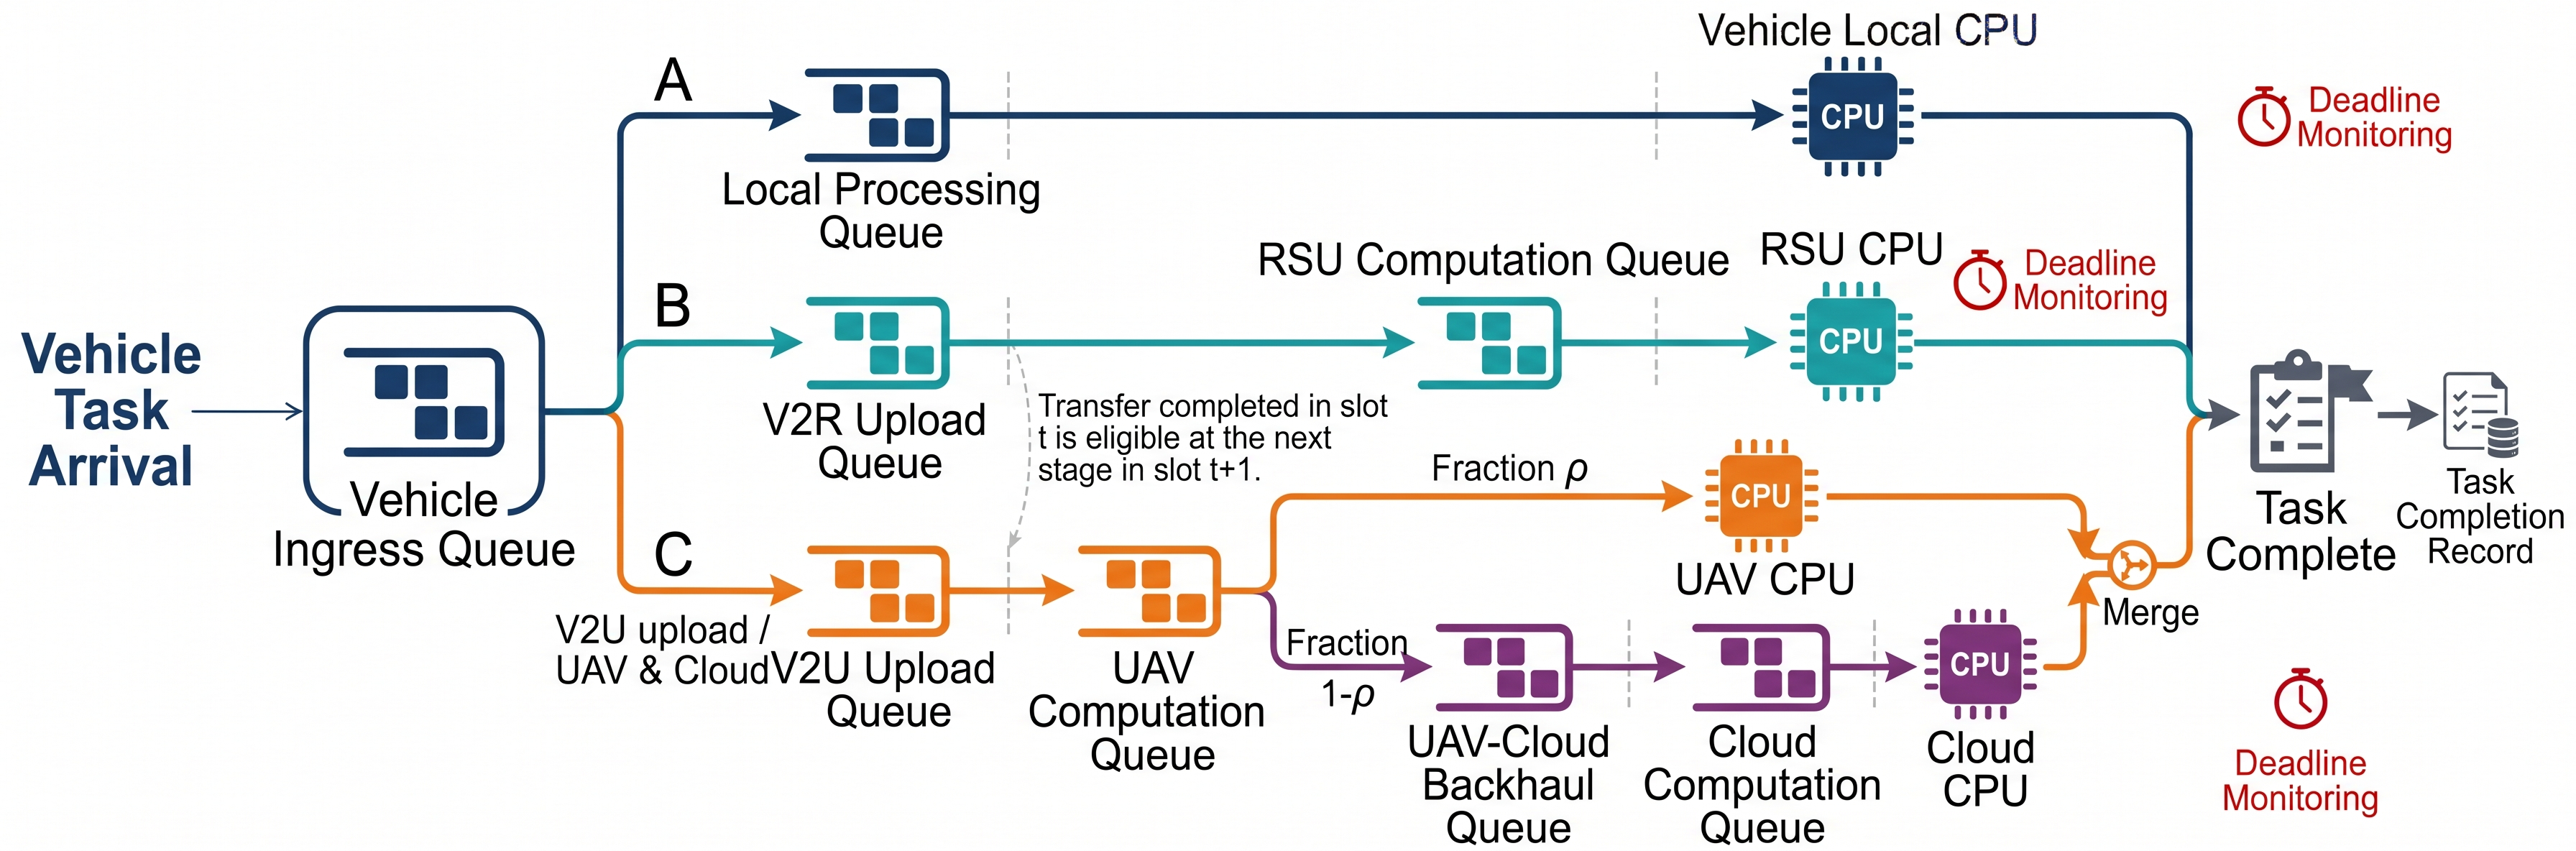
\includegraphics[width=0.96\textwidth]{End-to-end task lifecycle and queue mode.png}
\caption{End-to-end task service graph. Each box corresponds to a persistent
task or queue stage. A transfer committed at one boundary becomes eligible at
the next one.}
\label{fig:service_graph}
\end{figure*}

The core architecture leaves out a few options on purpose. There is no
direct vehicle-to-cloud or RSU-to-cloud route, tasks are not migrated between
UAVs, and nothing is reassigned after dispatch. Transmit powers are fixed and
the uplinks use orthogonal bandwidth. These restrictions let us study the
routing, CPU, split and trajectory decisions in isolation.

\begin{table*}[t]
\centering
\caption{Principal system notation.}
\label{tab:notation}
\renewcommand{\arraystretch}{1.12}
\begin{tabular}{p{0.13\textwidth}p{0.31\textwidth}p{0.13\textwidth}p{0.30\textwidth}}
\hline
\textbf{Symbol} & \textbf{Meaning} & \textbf{Symbol} & \textbf{Meaning}\\
\hline
$\Delta$ & Slot duration &
$\ell_i$ & Immutable task specification\\
$b_i,c_i,\chi_i$ & Input bits, CPU cycles, cycles per bit &
$a_i,d_i$ & Arrival time and deadline allowance\\
$Q_j(t)$ & Equivalent-cycle backlog of stage queue $j$ &
$A_j(t),S_j(t)$ & Realized queue arrival and service\\
$W_{ih}(t),R_{ih}(t)$ & Link bandwidth and transmission rate &
$f_n(t),w_{in}(t)$ & CPU frequency and task share\\
$B_k(t),H_k(t)$ & Physical UAV charge and harvested energy &
$Z_k(t)$ & Virtual net-energy deficit\\
$\boldsymbol p_v,\boldsymbol p_r,\boldsymbol p_k$ &
Vehicle, RSU, and UAV positions &
$\rho_i$ & UAV-local workload fraction\\
\hline
\end{tabular}
\end{table*}

\subsection{Vehicle Mobility and Coverage Model}
Synthetic vehicles drive along declared road polylines. The map
$\boldsymbol r_v(s)$ takes a route distance $s\in[0,L_v]$ to a 3-D road
coordinate, and $\nu_v(t)\ge0$ is the speed of the vehicle. Progress along the
route evolves as
\begin{equation}
\begin{aligned}
s_v(t+1)&=\mathscr R_v\!\left(
s_v(t)+\sigma_v(t)\nu_v(t)\Delta\right),\\
\boldsymbol p_v(t)&=\boldsymbol r_v(s_v(t)),
\end{aligned}
\label{eq:vehicle_motion}
\end{equation}
where $\sigma_v(t)\in\{-1,1\}$ gives the direction of travel and
$\mathscr R_v$ either wraps progress around a loop or reflects it at the end
of a route. In experiments with recorded SUMO traces,
Eq.~\eqref{eq:vehicle_motion} is replaced by the full sampled trace
$\boldsymbol p_v(t)=\boldsymbol p_v^{\mathrm{trace}}(t)$. Traces with missing
vehicle frames are rejected; we do not interpolate them.

For vehicle $v$ and edge node $n\in\mathcal R\cup\mathcal U$, the
three-dimensional distance and its horizontal component are
\begin{equation}
d_{vn}(t)=\|\boldsymbol p_v(t)-\boldsymbol p_n(t)\|,\qquad
d_{vn}^{\mathrm H}(t)=
\|[\boldsymbol p_v(t)-\boldsymbol p_n(t)]_{1:2}\|.
\label{eq:distances}
\end{equation}
Coverage is indicated by
$\mathbf 1\{d_{vr}^{\mathrm H}\le D_R\}$ for an RSU and by
$\mathbf 1\{d_{vk}^{\mathrm H}\le D_U\}$ for a UAV. We mask a destination if
it is out of coverage or inactive, if it is a UAV on its way back, or if no
admissible energy contingency exists for it.

\subsection{Task Generation, Lifecycle, and Offloading Model}
\label{subsec:task_model}
\subsubsection{Task Arrival and Persistent Record Model}
In slot $t$, vehicle $v$ produces $A_v^{\mathrm{task}}(t)$ jobs. For the
controlled synthetic benchmark we use
\begin{equation}
\begin{aligned}
A_v^{\mathrm{task}}(t)&\sim
\operatorname{Poisson}(\lambda_v(t)),\\
b_i&\in[b_{\min},b_{\max}],\quad
c_i\in[c_{\min},c_{\max}],\\
d_i&\in[d_{\min},d_{\max}],
\end{aligned}
\label{eq:task_arrival}
\end{equation}
where the draws are bounded and independent and are stored once in a
scenario trace. The low-load, near-capacity, overload, and surge cases are
distinguished through $\lambda_v(t)$. Every task carries the immutable record
\begin{equation}
\ell_i=(i,v(i),b_i,c_i,a_i,d_i,\zeta_i),\qquad
\chi_i=\frac{c_i}{b_i},
\label{eq:task_record}
\end{equation}
in which $\zeta_i\in\{0,1\}$ states whether the job can be partitioned.

\subsubsection{Destination Selection and Partitioning Model}
The indicator $h_i(t)$ means that the task is held in ingress, and $x_i^L(t)$,
$x_{ir}^R(t)$, and $x_{ik}^U(t)$ indicate dispatch to local execution, to an
RSU, and to a UAV. Before dispatch,
\begin{equation}
h_i(t)+x_i^L(t)+\sum_{r\in\mathcal R}x_{ir}^R(t)
 +\sum_{k\in\mathcal U}x_{ik}^U(t)=1,
\quad x,h\in\{0,1\}.
\label{eq:destination}
\end{equation}
With $h_i=1$ the task stays in ingress. As soon as any other choice is made,
the destination and the dispatch time can no longer change.

When a UAV is chosen, the whole input is uploaded to it first. The UAV then
executes a fraction $\rho_i$ of the work and forwards the rest to the cloud:
\begin{equation}
c_i^U=\rho_i c_i,\qquad
c_i^c=(1-\rho_i)c_i,\qquad
b_i^{\mathrm{bh}}=(1-\rho_i)b_i.
\label{eq:split}
\end{equation}
Indivisible work has $\rho_i=1$. For partitionable work, a value
$0\le\rho_i\le1$ is chosen at dispatch and then kept. A task is complete only
when every nonempty branch has finished and the merge delay
$\tau_i^{\mathrm{merge}}$ has passed.

\subsubsection{End-to-End Completion and Delay Model}
Given the actual completion time $f_i^{\mathrm{done}}$, the response time and
the deadline-success indicator are
\begin{equation}
T_i=f_i^{\mathrm{done}}-a_i,\qquad
\delta_i=\mathbf 1\{T_i\le d_i\}.
\label{eq:actual_latency}
\end{equation}
A miss is logged at the moment a task first crosses its deadline, and the
simulator keeps tracking the work that remains. A task that is still
unfinished when the trace ends is reported as censored, and we do not impute
a completion latency for it.

\subsection{Communication and OFDMA Service Model}
\subsubsection{Vehicle-to-RSU Terrestrial Channel Model}
On a vehicle--RSU link, the large-scale gain is deterministic:
\begin{equation}
g_{vr}^{R}(t)=g_0
\max\{d_{vr}(t),d_{\min}^{\mathrm{ch}}\}^{-\alpha_R},
\label{eq:rsu_gain}
\end{equation}
with reference gain $g_0$ and terrestrial path-loss exponent $\alpha_R$.

\subsubsection{Vehicle-to-UAV Air-to-Ground Channel Model}
On a vehicle--UAV link, the elevation angle and the LoS probability are
\begin{equation}
\begin{aligned}
\vartheta_{vk}(t)&=
\frac{180}{\pi}\tan^{-1}\!\left(
\frac{|z_k(t)-z_v(t)|}
{\max\{d_{vk}^{\mathrm H}(t),d_{\min}^{\mathrm{ch}}\}}\right),\\
p_{vk}^{\mathrm{LoS}}(t)&=
\left[1+a_{\mathrm L}
\exp\{-b_{\mathrm L}[\vartheta_{vk}(t)-a_{\mathrm L}]\}\right]^{-1}.
\end{aligned}
\label{eq:los}
\end{equation}
The mean aerial gain is then
\begin{equation}
\begin{aligned}
g_{vk}^{U}(t)={}&g_0
\max\{d_{vk}(t),d_{\min}^{\mathrm{ch}}\}^{-\alpha_U}\\
&\times\left[p_{vk}^{\mathrm{LoS}}\eta_{\mathrm L}
+(1-p_{vk}^{\mathrm{LoS}})\eta_{\mathrm N}\right],
\end{aligned}
\label{eq:uav_gain}
\end{equation}
in which the factors $\eta_{\mathrm L}=10^{-L_{\mathrm L}/10}$ and
$\eta_{\mathrm N}=10^{-L_{\mathrm N}/10}$ model the extra losses under LoS
and NLoS conditions.

\subsubsection{OFDMA Rate and Transmission-Service Model}
Suppose link $h$ is given bandwidth $W_{ih}(t)$ and has gain $g_{ih}(t)$,
and the vehicle transmits at fixed power $P_v^{\mathrm{tx}}$. Its rate is
then
\begin{equation}
R_{ih}(t)=W_{ih}(t)\log_2\!\left(
1+\frac{P_v^{\mathrm{tx}}g_{ih}(t)}
{N_0W_{ih}(t)+I_{ih}(t)}\right).
\label{eq:rate}
\end{equation}
Because the links are orthogonal, $I_{ih}=0$ and
$\sum_iW_{ih}\le W_h^{\max}$.

All controllers use the same deterministic scheduler, which assigns the
priority
\begin{equation}
\begin{aligned}
\pi_{ih}(t)&=q_{ih}^{\mathrm{eq}}(t)
\left[1+\min\left\{\frac{\operatorname{age}_i(t)}{d_i},
\kappa_{\mathrm{age}}\right\}\right],\\
W_{ih}(t)&=W_h^{\max}
\frac{\pi_{ih}(t)}{\sum_{\ell\in\mathcal E_h}\pi_{\ell h}(t)}.
\end{aligned}
\label{eq:ofdma}
\end{equation}
over the eligible links $\mathcal E_h$; exact ties are broken by task ID.
The term $q_{ih}^{\mathrm{eq}}$ is the backlog of the link expressed in
equivalent cycles. Any transfer of $s_{ih}^{\mathrm{tr}}$ equivalent cycles
has to satisfy
\begin{equation}
\sum_i\frac{s_{ih}^{\mathrm{tr}}(t)}{\chi_i}
\le\Delta R_h(t).
\label{eq:radio_capacity}
\end{equation}
A link that loses coverage serves nothing in that slot, and the bits it has
not yet sent stay in the upload queue where they started.

\subsection{Computation, Backhaul, and Queueing Model}
\subsubsection{Persistent Multi-Stage Queue Model}
The set $\mathcal J$ holds one queue per stage: ingress, V2R/V2U upload,
receive/staging, local/RSU/UAV compute, UAV backhaul, cloud receive, and
cloud compute. Queues measured in bits are converted to cycles only for the
drift accounting, with $b$ residual bits of task $i$ counted as $\chi_i b$
cycles.

Given the realized service $S_j(t)$ and arrivals $A_j(t)$, each queue $j$
evolves as
\begin{equation}
Q_j(t+1)=Q_j(t)-S_j(t)+A_j(t),\qquad
0\le S_j(t)\le Q_j(t).
\label{eq:queue}
\end{equation}
When a flow $F_{ab}(t)$ of equivalent work goes from stage $a$ to stage $b$,
it enters the increment of the source with a minus sign, $-F_{ab}$, and the
increment of the destination as $+F_{ab}$. Summing over all queues gives
\begin{equation}
\sum_{j\in\mathcal J}Q_j(t+1)=
\sum_{j\in\mathcal J}Q_j(t)+A^{\mathrm{ext}}(t)-C^{\mathrm{final}}(t),
\label{eq:conservation}
\end{equation}
apart from the branch creation and merge bookkeeping, which is logged
explicitly. Work is never lost through internal routing; it leaves the
system only when its final computation is done.

\subsubsection{CPU Service and Processor-Sharing Model}
For compute node $n$, the frequency $f_n$, the task shares $w_{in}$, and the
residual work that is ready, $c_{in}^{\mathrm{elig}}$, must satisfy
\begin{equation}
\begin{aligned}
0&\le f_n(t)\le f_n^{\max},\\
w_{in}(t)&\ge0,\qquad \sum_iw_{in}(t)\le1,\\
0\le s_{in}^{\mathrm{cpu}}(t)&\le
\min\{c_{in}^{\mathrm{elig}}(t),\Delta f_n(t)w_{in}(t)\}.
\end{aligned}
\label{eq:cpu_capacity}
\end{equation}
If a task finishes early, the capacity it leaves unused is shared out among
the other tasks that still have a positive share. In the core experiments,
scheduling on the vehicles and in the cloud is fixed, and so is the RSU clock
frequency. The controller sets the RSU task shares and, for each UAV, both the
frequency and the task shares.

\subsubsection{UAV Backhaul and Cloud-Service Model}
Before reaching the cloud, the cloud branch of a UAV task $i$ has to cross a
finite backhaul:
\begin{equation}
\sum_{i\in\mathcal B_k(t)}
\frac{s_{ik}^{\mathrm{bh}}(t)}{\chi_i}
\le\Delta R_k^{\mathrm{bh}},
\qquad
\sum_i s_{ic}^{\mathrm{cpu}}(t)\le\Delta f_c.
\label{eq:cloud_capacity}
\end{equation}
Once the backhaul transfer is done, $(1-\rho_i)c_i$ cycles are released to
cloud computation at the following boundary. The task is finished only when
both the UAV branch and the cloud branch (where nonempty) are complete.

\subsubsection{Queue-Stability Target}
We aim for the strong-stability condition
\begin{equation}
\limsup_{T\to\infty}\frac1T\sum_{t=0}^{T-1}
\mathbb E[Q_j(t)]<\infty,\qquad j\in\mathcal J.
\label{eq:stability}
\end{equation}
It only makes sense when the offered load can be stabilized, and in the
overload experiments we deliberately report the queue growth instead.

\subsection{UAV Movement and Collision-Avoidance Model}
With horizontal speed $v_k^{\mathrm H}$, azimuth $\theta_k$, and vertical
speed $v_k^z$, the velocity and the position are updated as
\begin{equation}
\begin{aligned}
\boldsymbol u_k(t)&=
\begin{bmatrix}
v_k^{\mathrm H}\cos\theta_k&
v_k^{\mathrm H}\sin\theta_k&v_k^z
\end{bmatrix}^{\mathsf T},\\
\boldsymbol p_k(t+1)&=\boldsymbol p_k(t)+\Delta\boldsymbol u_k(t).
\end{aligned}
\label{eq:uav_motion}
\end{equation}
A motion is admissible only if it stays within the speed, climb/descent,
map, altitude, and acceleration bounds:
\begin{equation}
\begin{aligned}
\|\boldsymbol u_k(t)\|&\le v_k^{\max},\\
-v_k^{\mathrm{down}}&\le v_k^z(t)\le v_k^{\mathrm{up}},\\
\|\boldsymbol u_k(t)-\boldsymbol u_k(t-1)\|&\le a_k^{\max}\Delta.
\end{aligned}
\label{eq:flight_bounds}
\end{equation}
Any two airborne UAVs must also keep their distance along the entire linear
trajectory of the slot:
\begin{equation}
\min_{\tau\in[0,\Delta]}
\|\boldsymbol p_k(t)+\tau\boldsymbol u_k(t)
-\boldsymbol p_l(t)-\tau\boldsymbol u_l(t)\|
\ge d_{\mathrm{safe}}.
\label{eq:collision}
\end{equation}
In addition, the controller keeps enough stopping distance from the map and
altitude boundaries. We call a return/landing plan verified when it consists
of segments that respect the same limits and ends at a declared landing site
with almost zero velocity.

\subsection{UAV and Infrastructure Energy-Consumption Models}
Fig.~\ref{fig:energy_safety_overview} gives an overview of the UAV energy
ledger, the replenishment paths, the flight constraints and the
return-reserve rule. Its laser-transfer branch is optional and was not active
in the stochastic-harvesting benchmark we report.

\begin{figure*}[!t]
\centering
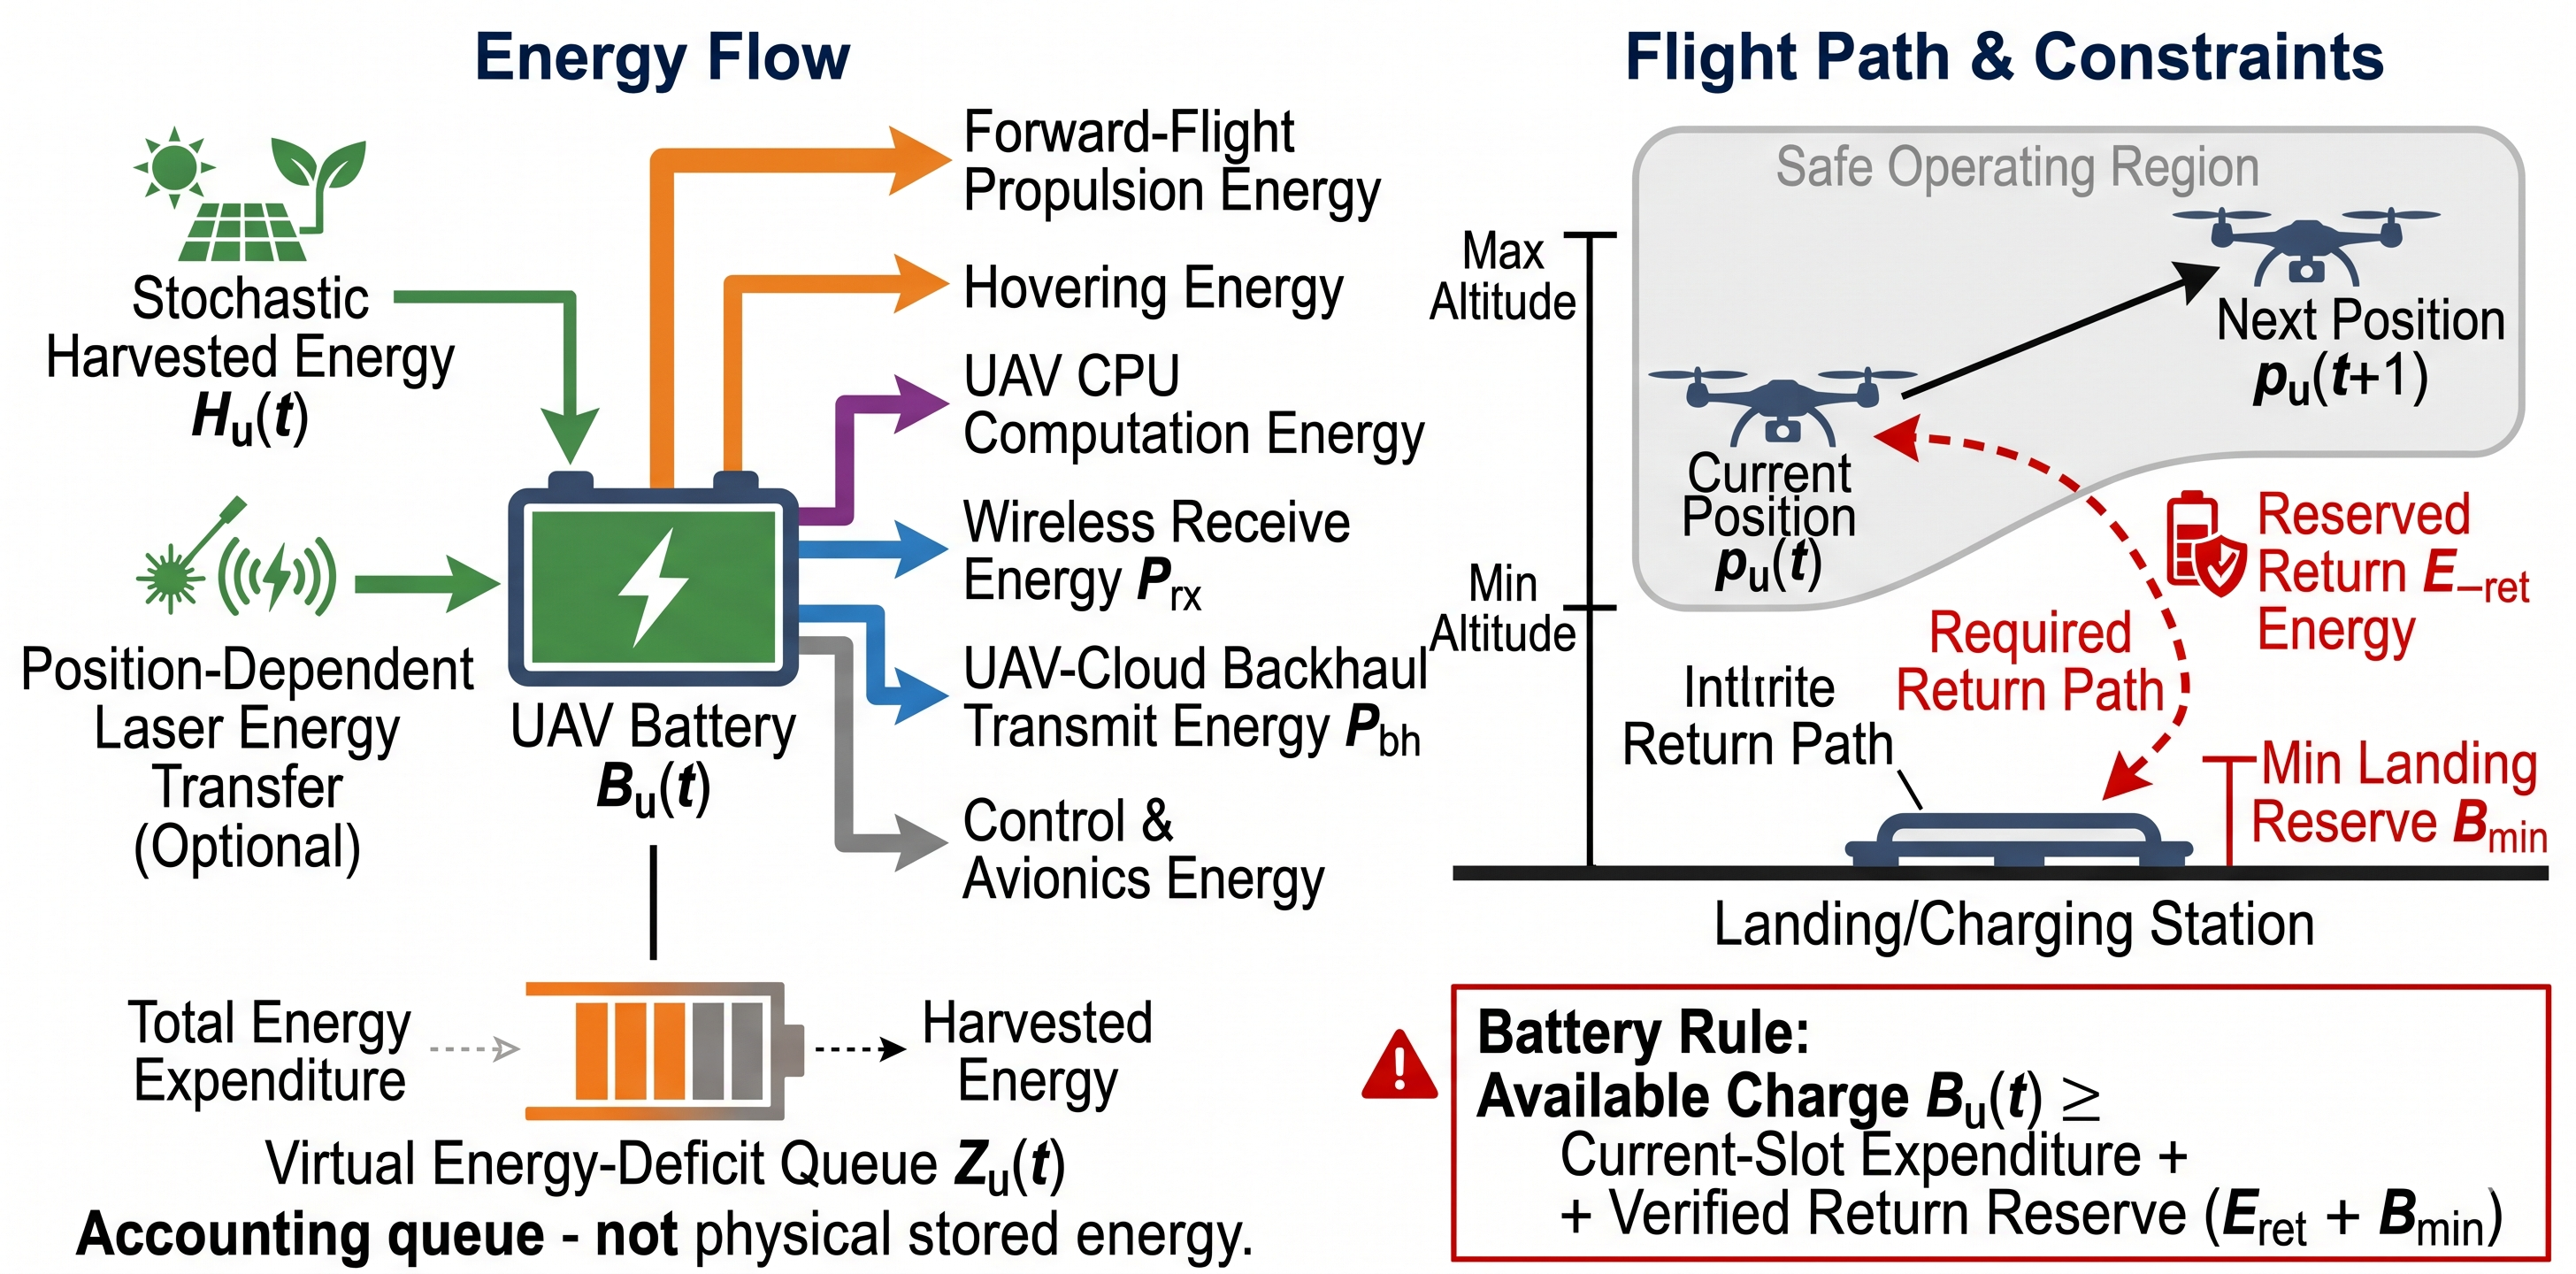
\includegraphics[width=0.94\textwidth]{UAV energy, harvesting, and return-reserve model.png}
\caption{UAV energy, harvesting, and return-reserve model. The physical
battery pays for propulsion, computation, communication, and control. Normal
service is allowed only while the current expenditure and a verified return
or landing reserve can both be met. The virtual deficit is a bookkeeping
queue; it does not store energy.}
\label{fig:energy_safety_overview}
\end{figure*}

\subsubsection{Rotary-Wing Flight and Hovering-Energy Model}
As in the energy accounting of~\cite{talukdar2026mappo}, the propulsion
ledger keeps motion and hovering apart. In slot $t$, let
$\tau_k^{\mathrm{fly}}(t)$ be the time spent in airborne flight and
$\tau_k^{\mathrm{hov}}(t)$ the time spent hovering at near-zero velocity,
where $\tau_k^{\mathrm{fly}}+\tau_k^{\mathrm{hov}}\le\Delta$. While flying,
the horizontal and vertical power is modeled as
\begin{equation}
\begin{aligned}
P_k^{\mathrm{fly}}={}&P_0\!\left(1+
\frac{c_p(v_k^{\mathrm H})^2}{U_{\mathrm{tip}}^2}\right)\\
&+P_i\!\left(\sqrt{1+\frac{(v_k^{\mathrm H})^4}{4v_0^4}}\right.\\
&\left.\hspace{3.1em}-\frac{(v_k^{\mathrm H})^2}{2v_0^2}\right)^{1/2}\\
&+c_d(v_k^{\mathrm H})^3
+c_{\uparrow}[v_k^z]^+
+c_{\downarrow}[-v_k^z]^+
+c_z(v_k^z)^2 .
\end{aligned}
\label{eq:propulsion}
\end{equation}
In this expression, $P_0$ is the blade-profile hover power and $P_i$ the
induced hover power, $U_{\mathrm{tip}}$ is the rotor-tip speed, and $v_0$ is
the mean induced velocity in hover. The other coefficients are calibrated and
capture horizontal drag as well as ascent and descent. When both the
horizontal and the vertical velocity are close to zero, the model reduces to
the hovering power
\begin{equation}
\begin{aligned}
P_k^{\mathrm{hov}}&=P_0+P_i,\\
E_k^{\mathrm{fly}}(t)&=P_k^{\mathrm{fly}}(t)
 \tau_k^{\mathrm{fly}}(t),\\
E_k^{\mathrm{hov}}(t)&=P_k^{\mathrm{hov}}
 \tau_k^{\mathrm{hov}}(t),\\
E_k^{\mathrm{prop}}(t)&=E_k^{\mathrm{fly}}(t)
 +E_k^{\mathrm{hov}}(t).
\end{aligned}
\label{eq:hovering}
\end{equation}
With this split, hover time is never billed a second time as flight. The present
implementation is piecewise constant over a slot: a nonzero airborne motion
command gives $(\tau_k^{\mathrm{fly}},\tau_k^{\mathrm{hov}})=(\Delta,0)$, and
an airborne hover gives $(0,\Delta)$. Writing the two intervals separately
leaves room for sub-slot scheduling later on. Any remaining part of the slot
belongs to a landed or otherwise non-airborne mode, for which the airborne
propulsion power is zero. We note that Eq.~\eqref{eq:propulsion} is a
calibrated approximation for bounded flight and not a complete aerodynamic
model.

\subsubsection{Computation and Communication-Energy Model}
UAV $k$ computes $s_k^{\mathrm{cpu}}$ cycles. While it receives uplink data
from vehicles, its receiver chain draws power $P_k^{\mathrm{rx}}$ over an
active reception time $\tau_k^{\mathrm{rx}}$. In the same way, the UAV
transmits on the UAV--cloud backhaul with power $P_k^{\mathrm{bh}}$ for an
active time $\tau_k^{\mathrm{bh}}$. The avionics and control electronics,
which run whenever the UAV is active, are covered by $P_k^{\mathrm{ctrl}}$
and $\tau_k^{\mathrm{ctrl}}$. All powers are in watts and all active times in
seconds, so each product is an energy in joules. The individual energy terms
are
\begin{equation}
\begin{aligned}
E_k^{\mathrm{cpu}}&=\kappa_k f_k^2s_k^{\mathrm{cpu}},\\
E_k^{\mathrm{rx}}&=P_k^{\mathrm{rx}}\tau_k^{\mathrm{rx}},&
E_k^{\mathrm{bh}}&=P_k^{\mathrm{bh}}\tau_k^{\mathrm{bh}},\\
E_k^{\mathrm{ctrl}}&=P_k^{\mathrm{ctrl}}\tau_k^{\mathrm{ctrl}}.&&
\end{aligned}
\label{eq:energy_components}
\end{equation}
Adding these terms, the total UAV expenditure is
\begin{equation}
E_k=E_k^{\mathrm{fly}}+E_k^{\mathrm{hov}}+E_k^{\mathrm{cpu}}
+E_k^{\mathrm{rx}}+E_k^{\mathrm{bh}}+E_k^{\mathrm{ctrl}}.
\label{eq:uav_energy}
\end{equation}
A vehicle spends $P_v^{\mathrm{tx}}\tau_v^{\mathrm{tx}}$ on its uplink. The
compute energy of RSUs and of the cloud follows the same
$\kappa_nf_n^2s_n^{\mathrm{cpu}}$ rule, and their receiver energy is charged
separately. In the system energy, each ownership component is counted once.

\subsection{Energy-Harvesting, Battery, and Return-Reserve Model}
\subsubsection{Stochastic Energy-Replenishment Model}
In the implementation, energy is replenished according to the trace
\begin{equation}
H_k(t)=I_k^{\mathrm{src}}(t)\,\bar H_k\,\xi_k(t),\qquad
\xi_k(t)\sim\mathcal U[1-\delta_H,1+\delta_H],
\label{eq:stochastic_harvest}
\end{equation}
with $I_k^{\mathrm{src}}(t)=0$ during a declared outage and
$I_k^{\mathrm{src}}(t)=1$ at all other times. We use $\delta_H=0.2$ in the benchmark and set
$\bar H_k=0$ in the zero-harvest scenarios. Each realization is drawn once,
and all compared controllers see the same one.

\subsubsection{Optional Position-Dependent Laser-Transfer Model}
Should a laser source located at $\boldsymbol p_L$ be added later, the
following optional model makes the harvested energy depend on position:
\begin{equation}
\begin{aligned}
d_{Lk}(t)&=\|\boldsymbol p_k(t)-\boldsymbol p_L\|,\\
P_k^{\mathrm{rec}}(t)&=
P_L(t)\frac{A_k}{[\theta_Ld_{Lk}(t)]^2}
\exp[-\kappa_{\mathrm{atm}}(t)d_{Lk}(t)]
\eta_k^{\mathrm{align}}(t),\\
H_k^{\mathrm{laser}}(t)&=\Delta\eta_k^{\mathrm{pv}}
P_k^{\mathrm{rec}}(t).
\end{aligned}
\label{eq:optional_laser}
\end{equation}
Using it would require calibrated values for the beam divergence, atmospheric
attenuation, alignment, aperture, and photovoltaic efficiency. The current
stochastic benchmark does not include it.

\subsubsection{Battery Evolution, Energy Causality, and Landing Reserve}
We write $B_k^{\mathrm{pre}}(t+1)$ for the charge left right after the
slot's expenditure and before the end-of-slot replenishment. The battery then
obeys
\begin{equation}
\begin{aligned}
B_k^{\mathrm{pre}}(t+1)&=B_k(t)-E_k(t),\\
B_k(t+1)&=\min\{B_k^{\max},
B_k^{\mathrm{pre}}(t+1)+H_k(t)\},\\
0&\le B_k(t)\le B_k^{\max},\qquad
0\le E_k(t)\le B_k(t).
\end{aligned}
\label{eq:battery}
\end{equation}
This ordering means that harvested energy becomes usable only after the
current expenditure has been paid; it cannot fund an action taken earlier in
the same slot. To
combine a declared emergency floor with a return-safety margin that depends
on the state, we define
$B_k^{\min}=\xi_kB_k^{\max}$ for $\xi_k\in[0,1)$ when such a floor is
specified (and $B_k^{\min}=0$ otherwise), and
\[
B_k^{\mathrm{safe}}(t+1)=\max\!\left\{B_k^{\min},
B_k^{\mathrm{res}}(\boldsymbol p_k(t+1),\boldsymbol u_k(t))\right\}.
\]
During normal service, the following stronger energy-causality constraint
must hold:
\begin{equation}
B_k^{\mathrm{pre}}(t+1)\ge B_k^{\mathrm{safe}}(t+1).
\label{eq:reserve}
\end{equation}
The quantity $B_k^{\mathrm{res}}$ is the energy needed for a verified
return/landing plan, computed without counting on any future harvest. Battery
overflow, $O_k(t)=[B_k^{\mathrm{pre}}(t+1)+H_k(t)-B_k^{\max}]^+$, is logged
but not credited as usable energy. If a UAV cannot keep
Eq.~\eqref{eq:reserve} satisfied, it switches to a verified return/landing
contingency, and UAVs that are returning or have landed cannot be chosen as
new destinations.

\section{Problem Formulation}
\label{problem_formulation}

The component models are linked through four kinds of controller decision:
dispatch, partitioning, CPU allocation and UAV motion. This section first
defines the per-slot cost used by the learning and Lyapunov layers and then
states the long-term stochastic optimization problem, with every physical
constraint written out.

\subsection{Instantaneous Cost Model}
Let $N(t)$ be the number of unfinished tasks and $M(t)$ the number of tasks
that cross their deadline for the first time in slot $t$. We use the
normalized instantaneous cost
\begin{equation}
C(t)=w_L\frac{\Delta N(t)}{L_{\mathrm{ref}}}
+w_E\frac{E^{\mathrm{sys}}(t)}{E_{\mathrm{ref}}}
+w_DM(t).
\label{eq:cost}
\end{equation}
The references are fixed so that costs can be compared between scenarios.
For a drained trace, the summed occupancy approximates the aggregate sojourn
time; the latency we report, however, is always computed from
Eq.~\eqref{eq:actual_latency}.

\subsection{Long-Term Stochastic Optimization Problem}
The vector $\boldsymbol\alpha(t)$ gathers every dispatch, split, CPU, and
motion decision. To keep the notation short, we write
$\mathcal D_i=\{L(i)\}\cup\mathcal R\cup\mathcal U$ for the candidate
destinations of task $i$ and use $m_{in}(t)\in\{0,1\}$ to show whether
destination $n$ is open to this task in slot $t$. The mask is set to zero for
a link without coverage, for a UAV that is returning or has landed, and for
any destination that fails the physical safety checks. The long-run problem
reads
\begin{equation}
\begin{aligned}
\mathcal P:\quad \min_{\pi}\;&
\limsup_{T\to\infty}\frac1T
\sum_{t=0}^{T-1}\mathbb E_{\pi}[C(t)].
\end{aligned}
\label{eq:problem}
\end{equation}
Instead of folding feasibility into a single set symbol, we list the
constraints one by one below. Unless another quantifier is given, each must
hold in every slot and for every task, applicable node, and UAV.

\stepcounter{equation}
\begin{equation}
\begin{gathered}
h_i(t)+\sum_{n\in\mathcal D_i}x_{in}(t)=1,\\
h_i(t),x_{in}(t)\in\{0,1\}
\end{gathered}
\tag{C1}\label{con:routing}
\end{equation}
\stepcounter{equation}
\begin{equation}
x_{in}(t)\le m_{in}(t),\qquad n\in\mathcal D_i
\tag{C2}\label{con:mask}
\end{equation}
\stepcounter{equation}
\begin{equation}
0\le\rho_i(t)\le1,\qquad
\rho_i(t)=1\ \text{if }\zeta_i=0
\tag{C3}\label{con:split}
\end{equation}
By (C1), a task is either held, executed locally, offloaded to an RSU, or
offloaded to a UAV, and exactly one of these applies. (C2) rules out dispatch
over a link that is unavailable or to a UAV that is unsafe. (C3) allows a
cloud split only when the task is partitionable. After dispatch, the chosen
destination and split do not change.

\stepcounter{equation}
\begin{equation}
\begin{gathered}
s_{ih}^{\mathrm{tr}}(t)\ge0,\qquad
\sum_i\frac{s_{ih}^{\mathrm{tr}}(t)}{\chi_i}\le\Delta R_h(t),\\
W_{ih}(t)\ge0,\qquad \sum_iW_{ih}(t)\le W_h^{\max}
\end{gathered}
\tag{C4}\label{con:radio}
\end{equation}
\stepcounter{equation}
\begin{equation}
\begin{gathered}
0\le f_n(t)\le f_n^{\max},\qquad w_{in}(t)\ge0,\\
\sum_iw_{in}(t)\le1
\end{gathered}
\tag{C5}\label{con:processor}
\end{equation}
\stepcounter{equation}
\begin{equation}
0\le s_{in}^{\mathrm{cpu}}(t)\le
\min\{c_{in}^{\mathrm{elig}}(t),\Delta f_n(t)w_{in}(t)\}
\tag{C6}\label{con:cpu-service}
\end{equation}
\stepcounter{equation}
\begin{equation}
\begin{gathered}
\sum_{i\in\mathcal B_k(t)}\frac{s_{ik}^{\mathrm{bh}}(t)}{\chi_i}
\le\Delta R_k^{\mathrm{bh}},\\
\sum_i s_{ic}^{\mathrm{cpu}}(t)\le\Delta f_c
\end{gathered}
\tag{C7}\label{con:backhaul-cloud}
\end{equation}
\stepcounter{equation}
\begin{equation}
\begin{gathered}
0\le S_j(t)\le Q_j(t),\\
Q_j(t+1)=Q_j(t)-S_j(t)+A_j(t)
\end{gathered}
\tag{C8}\label{con:queue-causality}
\end{equation}
The limits on spectrum, processors, backhaul, the cloud, and queue service
are given by (C4)--(C8). In particular, a stage cannot serve more work than was
eligible when the slot began. Output from an upstream stage joins the
downstream queue only at the next slot boundary, so a task cannot pass
through several stages within one slot.

With $\mathcal A$ the horizontal operating region, the UAVs are subject to
\stepcounter{equation}
\begin{equation}
\begin{gathered}
\boldsymbol p_k(t+1)=\boldsymbol p_k(t)+\Delta\boldsymbol u_k(t),\\
\boldsymbol p_k^{\mathrm H}(t+1)\in\mathcal A,\qquad
z_k^{\min}\le z_k(t+1)\le z_k^{\max}
\end{gathered}
\tag{C9}\label{con:position}
\end{equation}
\stepcounter{equation}
\begin{equation}
\begin{gathered}
\|\boldsymbol u_k(t)\|\le v_k^{\max},\\
-v_k^{\mathrm{down}}\le u_k^z(t)\le v_k^{\mathrm{up}}
\end{gathered}
\tag{C10}\label{con:speed}
\end{equation}
\stepcounter{equation}
\begin{equation}
\|\boldsymbol u_k(t)-\boldsymbol u_k(t-1)\|
\le a_k^{\max}\Delta
\tag{C11}\label{con:acceleration}
\end{equation}
\stepcounter{equation}
\begin{equation}
\begin{aligned}
\min_{\tau\in[0,\Delta]}\|&\boldsymbol p_k(t)+\tau\boldsymbol u_k(t)\\
&-\boldsymbol p_l(t)-\tau\boldsymbol u_l(t)\|
\ge d_{\mathrm{safe}},\quad k\ne l
\end{aligned}
\tag{C12}\label{con:separation}
\end{equation}
Constraints (C9)--(C12) cover the kinematics, the flight region, altitude,
speed, climb and descent rates, acceleration, and separation along the
continuous path. The stopping distance a UAV needs to stay inside the region
is built into the feasibility mask of (C2); it is not something checked only
after the motion has been carried out.

\stepcounter{equation}
\begin{equation}
\begin{gathered}
B_k^{\mathrm{pre}}(t+1)=B_k(t)-E_k(t),\\
B_k(t+1)=\min\{B_k^{\max},B_k^{\mathrm{pre}}(t+1)+H_k(t)\},\\
0\le B_k(t+1)\le B_k^{\max}
\end{gathered}
\tag{C13}\label{con:battery-dynamics}
\end{equation}
\stepcounter{equation}
\begin{equation}
\begin{gathered}
0\le E_k(t)\le B_k(t),\\
B_k^{\mathrm{pre}}(t+1)\ge B_k^{\mathrm{safe}}(t+1)
\end{gathered}
\tag{C14}\label{con:energy-reserve}
\end{equation}
\stepcounter{equation}
\begin{equation}
\limsup_{T\to\infty}\frac1T\sum_{t=0}^{T-1}
\mathbb E_{\pi}[Q_j(t)]<\infty,\quad j\in\mathcal J
\tag{C15}\label{con:queue-stability}
\end{equation}
\stepcounter{equation}
\begin{equation}
\limsup_{T\to\infty}\frac1T\sum_{t=0}^{T-1}
\mathbb E_{\pi}[E_k(t)-H_k(t)]\le\bar e_k,\quad k\in\mathcal U
\tag{C16}\label{con:average-energy}
\end{equation}
\stepcounter{equation}
(C13) and (C14) encode the implemented timing, in which energy is spent
before the harvest arrives, together with the battery capacity (through the
clipped update), immediate energy causality, and the verified return/landing
reserve. (C15) is the strong-stability target for each physical queue; in the
tests that are overloaded on purpose, we measure whether it holds and do not
assume it. In (C16), choosing $\bar e_k=0$ asks for energy neutrality over
the long run, while $\bar e_k>0$ allows a declared average battery draw over
a finite mission. Deadlines enter the cost through $M(t)$. Imposing them as
hard constraints could make the problem infeasible, and a task that misses its
deadline simply stays in the physical queues until it is completed.
